\begin{frame}{The Standard Model of Particle Physics}
  \framesubtitle{-}

  \begin{columns}

    \begin{column}{0.5\textwidth}

      \begin{figure}
        \centering
        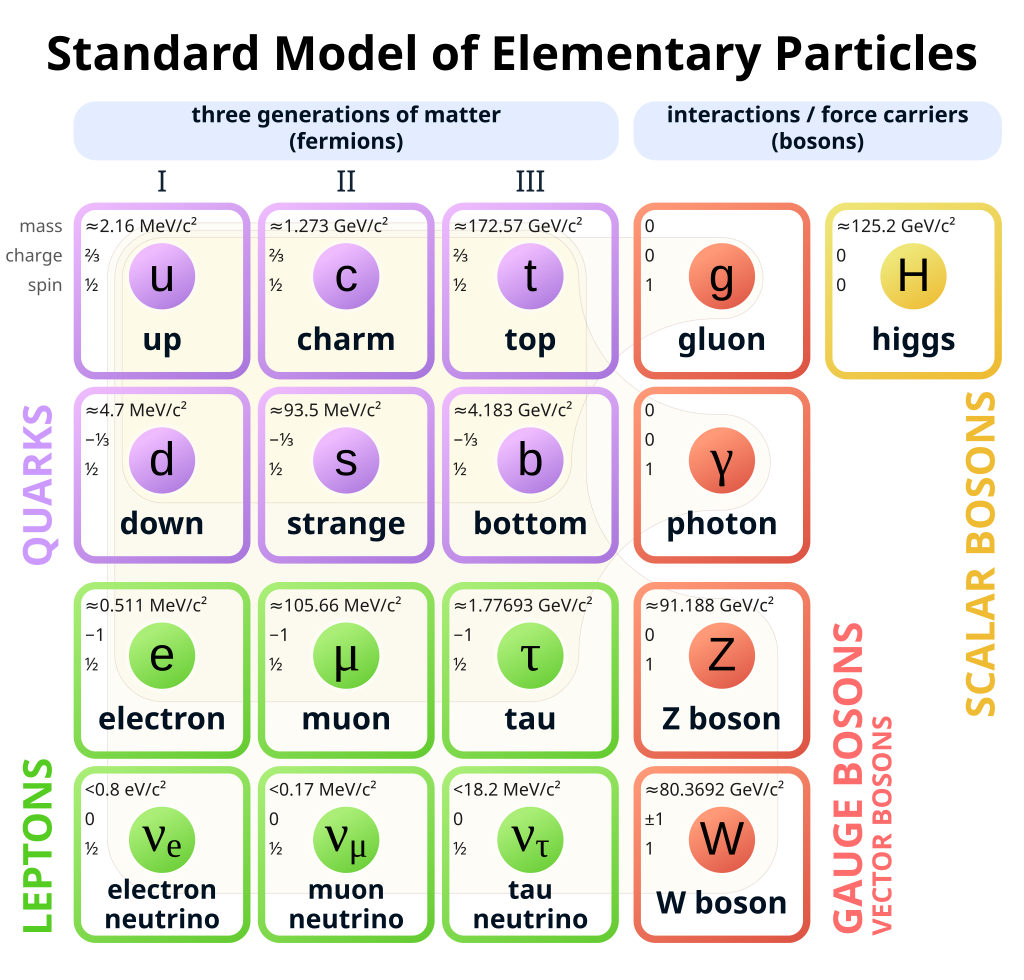
\includegraphics[width = \textwidth]{imgs/standard-model.png}
      \end{figure}

    \end{column}

    \begin{column}{0.5 \textwidth}

      \begin{colorblock}[white]{stataleyellow}{Main BSM evidence}
        \begin{itemize}
          \item dark matter and dark energy
          \item matter-antimatter asymmetry
          \item neutrino masses
        \end{itemize}
      \end{colorblock}

      \vspace{0.5em}


      \capcol{Figure} from Clowe et al. 2006.

      \justifying
      Offset between the observed baryonic mass distribution and the gravitational potential in the Bullet Cluster (1E 0657-56).

    \end{column}

  \end{columns}

\end{frame}

%=======================================================================

\begin{frame} {Collider Physics}
  \framesubtitle{One of the principal methods of research}
  
\end{frame}

